

- We trained classifiers using more and more principle components to decode,
and compared across condi- tions with varying degrees of cognitive richness.

-We found that as listening conditions become more cognitively rich, decoding
accuracy increased.

-Also, decoding accuracy increased as understanding of the narrative
accumulated over time, in more complex listening conditions.

- Decoding accuracy also increased in higher cognitive areas, in more complex
listening conditions. -We found that as story listening conditions become more
complex, more components are required to decode.

-We also found we could decode better with more impoverished data when there is
the underlying structure of the narrative providing more cognitive richness.

-We posit that as the complexity of our thoughts increases, neural compression
decreases. However, as our thoughts become deeper and richer, more reliable
information is available at higher neural compression.







Based on prior work ~\citep{Deme19} and following the direction of the field
~\citep{Turk13} we think our thoughts might be encoded in dynamic network
patterns, and possibly higher order network patterns
(Fig.~\ref{fig:direction_of_field}). We sought to test this hypothesis by
developing an approach to inferring high-order network dynamics from timeseries
data.

One challenge in studying dynamic interactions is the computational resources
required to calculate higher-order correlations. We developed a computationally
tractable model of network dynamics (Fig.~\ref{fig:methods_fig}) that takes in
a feature timeseries and outputs approximated first-order dynamics (i.e.,
dynamic functional correlations), second-order dynamics (reflecting homologous
networks that dynamically form and disperse), and higher-order network dynamics
(up to tenth-order dynamic correlations).

We first validated our model using synthetic data, and explored how recovery
varied with different underlying data structures and kernels. We then applied
the approach to an fMRI dataset ~\citep{SimoEtal16} in which participants
listened to an audio recording of a story, as well as scrambled versions of the
same story (where the scrambling was applied at different temporal scales). We
trained classifiers to take the output of the model and decode the timepoint in
the story (or scrambled story) that the participants were listening to. We
found that, during the intact listening condition in the experiment,
classifiers that incorporated higher-order correlations yielded consistently
higher accuracy than classifiers trained only on lower-order patterns
(Fig.~\ref{fig:decoding_level}, a.\&d.). By contrast, these higher-order
correlations were not necessary to support decoding the other listening
conditions and (minimally above chance) during a control rest condition. This
suggests that the cognitive processing that supported the most cogntively rich
listening conditions involved second-order (or higher) network dynamics.

Although we found decoding accuracy was best when incorporating higher-order
network dynamics for all but rest condition, it is unclear if this is a product
of the brain or the data collection technique. It could be that the brain is
second-order or it could be that fMRI can only reliably give second-order
interactions. Exploring this method with other data collection technique will
be important to disentangle this question.



  \subsection*{Concluding remarks}

How can we better understand how brain patterns change over
time? How can we quantify the potential network dynamics that might be
driving these changes? One way to judge the techniques of the future is
to look at the trajectory of the fMRI field so far has taken so far
(Fig.~\ref{fig:methods_fig}).  The field started with 
univariate activation, measuring the average activity for each voxel.
Analyses of multivariate activation followed, looking at spatial patterns of
activity over voxels. Next, correlations of activity were explored, first
with measures like resting connectivity that take temporal correlation
between a seed voxel and all other voxels then with full connectivty
that measure all pairwise correlations.  Additionally, this path of increasing
complexity also moved from static to dynamic measurements.  One
logical next step in this trajectory would be dynamic higher-order
correlations. We have created a method 
to support these calculations by scalably approximating dynamic higher-order
correlations.  









By training classifiers using more and more principle components to decode, and
comparing across conditions with varying degrees of cognitive richness, we can
assess the explanatory power of the compressed data held with respect to the
observed data (see \textit{Methods}). We note that our primary goal was not to
achieve perfect decoding accuracy, but rather to use decoding accuracy as a
benchmark for assessing whether different neural features specifically capture
cognitively relevant brain patterns.

\begin{figure} \centering
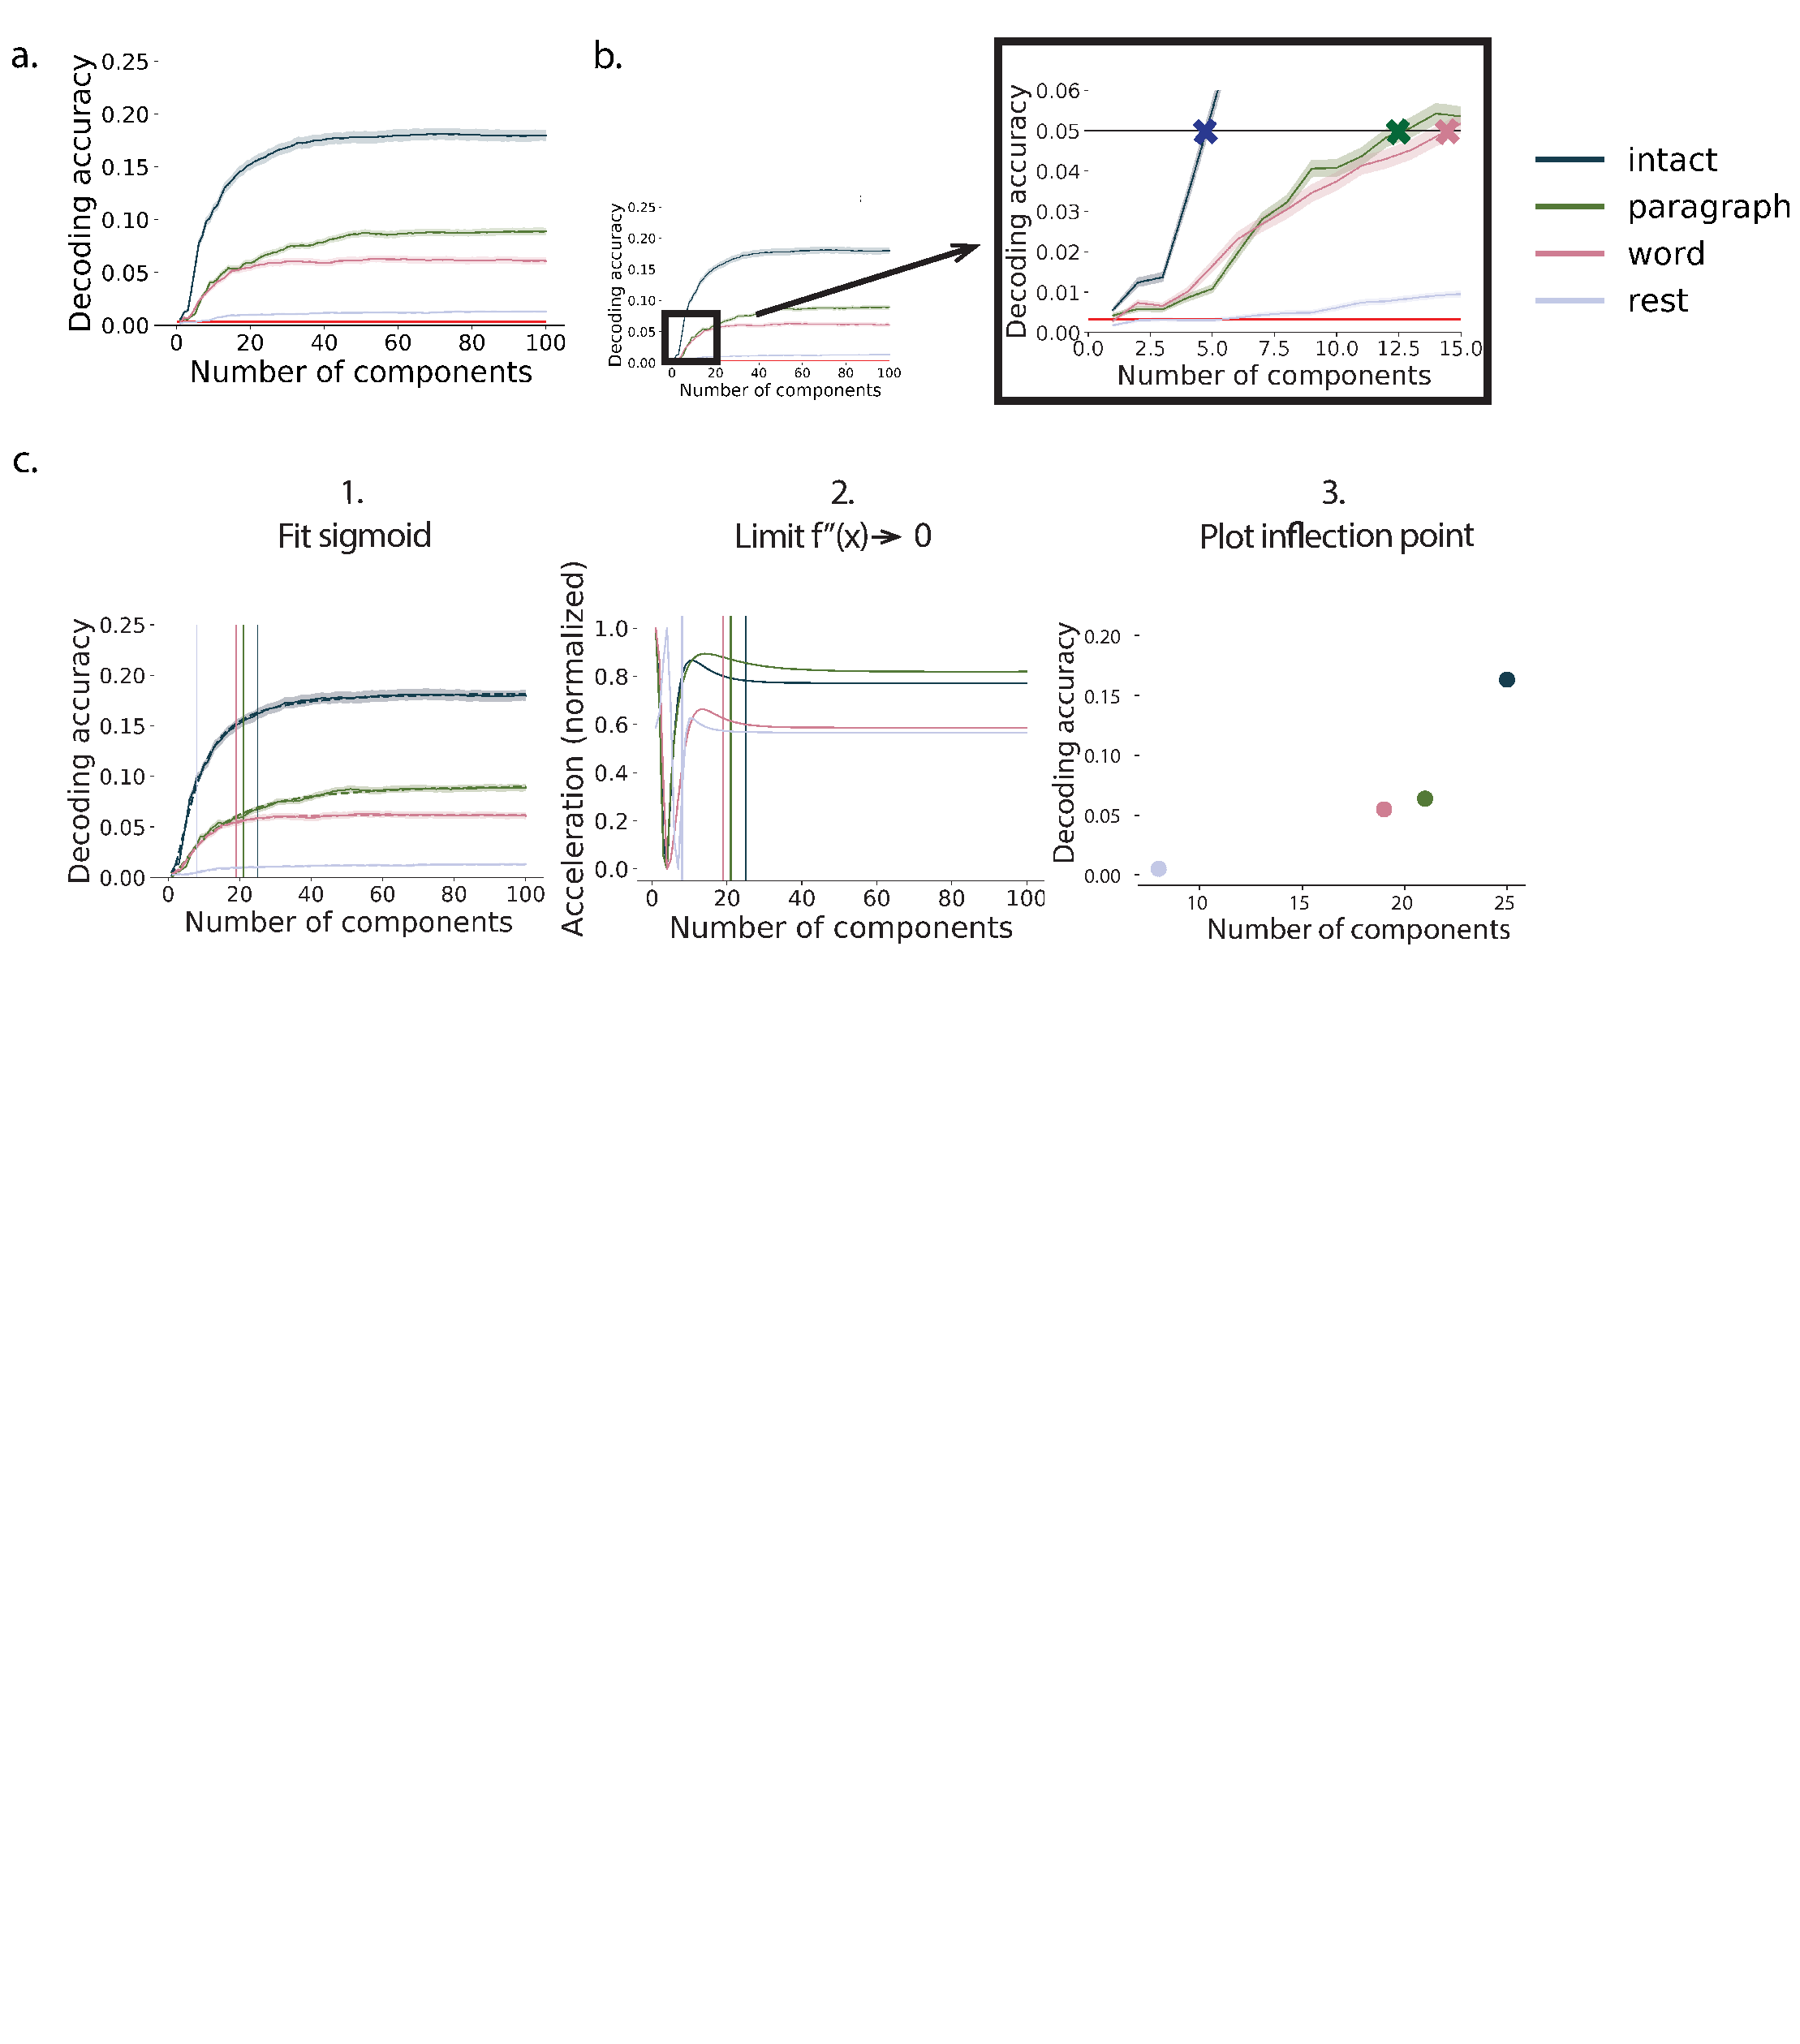
\includegraphics[width=\textwidth]{figs/decode_interpret.pdf}
\caption{\textbf{Decoding accuracy.} \textbf{a. Decoding accuracy by number of
components.} Ribbons of each color display cross-validated decoding performance
for each condition (intact, paragraph, word, and rest). Decoders were trained
using increasingly more principle components and displayed relative to chance
(red line). \textbf{b. Fixed decoding accuracy by number of components.} We
zoom in on the plot shown in \textbf{a.} and add a line denoting fixed decoding
accuracy (.05). We plot where the intact, paragraph, and word conditions
intersect. \textbf{c. Explanation of inflection metric.} First the we fit a
sigmoid function to the decoding accuracy by number of components. Second, we
found where the second derivative is both positive and less than .0001. Last,
we then plot that inflection point as a single metric to capture the slope and
asymptote of the curve.} \label{fig:decode_interpret} \end{figure}




  We also wondered how this compression would change across brain regions. We
  repeated the analysis but limited the brain hubs to 7 networks using the Yeo
  et al. (2011) network parcellation shown here in the inflated brain
  (Fig.~\ref{fig:decode_pcs_network}, d.). We found that as complexity of the
  stimuli increases, decoding accuracy increases with higher cognitive areas.
  (Fig.~\ref{fig:decode_pcs_network}).





We were also curious how compression would change across time. If, there is
some understanding of the narrative that accumulates over time, we should be
able to see that difference. We found increases in decoding accuracy with the
same number or fewer components for more complex, cognitively rich, conditions.
We also found decreases in decoding accuracy for the word-scrambled and rest
condition.

Overall, we found that as story listening conditions become more complex, more
components are required to decode. We also found we could decode better with
more impoverished data when there is the underlying structure of the narrative
providing more cognitive richness. We posit that as the complexity of our
thoughts increases, neural compression decreases. However, as our thoughts
become deeper and richer, more reliable information is available at higher
neural compression.



% - Increases in decoding accuracy with the same number or fewer components for
more complex, cognitively rich, conditions. % - Decreases in decoding accuracy
for the word-scrambled and rest % condition.


%%%%%%%%%%%%%%%%%%%%%%%%%%%%%%%%%%%%%%%
  
  
  % As complexity of the stimuli increases, decoding accuracy increases
  % with higher cognitive areas. (Fig.~\ref{fig: decode_pcs_network}).
  
  % If, there is some understanding of the narrative that accumulates over
  time, we should be able to see that change.
  



% We performed a decoding analysis, using cross validation to estimate % (using
other participants’ data) which parts of the story the additional added %
principle component corresponded to (see \textit{Materials and methods}). We
note that our primary goal was not to achieve perfect decoding accuracy, but
rather to use decoding accuracy as a benchmark for assessing whether different
neural features specifically capture cognitively relevant brain patterns.

% Separately for each experimental condition, we divided participants % into
two groups. Starting with 1 principle comonent, for % each dimension we added
another principle component, and we correlated the group 1 activity patterns
with group 2 % activity patterns. There were 272 % timepoints for paragraph
condition, 300 timepoints for intact and word % conditions, and 400 timepoints
for rest condition, so chance % performance on this decoding test is was
$\frac{1}{272}$, % $\frac{1}{300}$, and $\frac{1}{400}$ respectively.
 
% - As complexity of the stimulus increases, decoding accuracy % increases
(Fig.~\ref{fig:decode_interpret}, a.). Replication of % Simony findings.

% - As complexity of the stimuli increases, we need fewer components to %
decode the same amount (Fig.~\ref{fig:decode_interpret}, b.).

% - As complexity of the stimuli increases, more components are required to
reach peak decoding accuracy (Fig.~\ref{fig:decode_interpret}, c.).




Prior work has shown participants share similar neural responses to richly
structured stimuli when compared to stimuli with less structure
\cite{SimoEtal16}. We replicate this finding, showing as complexity of the
stimulus increases, decoding accuracy increases
(Fig.~\ref{fig:decode_interpret}, a.). Additionally, we found that as
complexity of the stimuli increases, we need fewer components to decode the
same amount (Fig.~\ref{fig:decode_interpret}, b.). However, we also found that
as complexity of the stimuli increases, more components are required to reach
peak decoding accuracy (Fig.~\ref{fig:decode_interpret}, c.). We posit that as
the complexity of our thoughts increases, neural compression decreases.
However, as our thoughts become deeper and richer, more reliable information is
available at higher neural compression.


% % PCA, or the closely related factor analysis and singular value
decomposition (SVD) (Hastie et al., 2009), is widely used in the study of
individual differences and aids estimating how many latent components, or
“factors”, underlie a pattern of (item) responses within or across
participants, as for instance in the context of intelligence (Spearman, 1904)
or personality tests (Cattell, 1947). In the context of neuroimaging, PCA has
been used to identify brain networks (Huth et al., 2012; Friston et al., 1993).

% % add citation: % % S.M.Smith,A.Hyva ̈rinen,G.Varoquaux,K.L.Miller,and C. F.
Beckmann, “Group-PCA for very large fMRI datasets,” NeuroImage, vol. 101, pp.
738, 2014.


% \subsection*{Evaluation metrics} % We will evaluate the degree of %
compression of held-out % neuroimaging data by assessing the time at which it
was collected. We will use this evaluation (timepoint % decoding) as a proxy
for % gauging how much explanatory power the compressed data held % with
respect to the observed data.



% \subsubsection*{Timepoint decoding}

% To explore how compression varies with complexity, we will use a previous neuroimaging dataset
% ~\cite{SimoEtal16}  in which participants listened to an audio recording of a story; 36 particpants listen to an intact version of the story, 17 participants listen to time-scrambled recordings of the same story where paragraphs were scrambled, 36 particpants listen to word-scrambled version and 36 participants lay in rest condition.


% Following the analyses conducted by (HTFA)~\cite{MannEtal18}, we first
% apply \textit{hierarchical topographic factor analysis} (HTFA) to
% the fMRI datasets to obtain a time series of 700 node activities for
% every participant.  We then apply dimensionality reduction
% (Incremental PCA) for each group.

% We then compare the groups’ activity patterns (using Pearson
% correlations) to estimate the story times each corresponding pattern
% using more and more principle components.   

% To assess decoding accuracy, we randomly divide participants for each
% stimulus into training and testing groups. We then compare the
% groups’ activity patterns (using Pearson correlations) to estimate the
% story times each corresponding pattern using more and more principle
% components (as the data became less compressed). Specifically, we ask, for each timepoint: what are the correlations
% between the first group's and second group's activity patterns at each
% order. We note that the decoding test we used is a conservative in which we count a timepoint label as incorrect if it is not an exact match.





% \subsection*{Evaluation metrics}
%  We evaluated the degree of
% compression of held-out
% neuroimaging data with the time at which it was collected.  We used this latter evaluations (using timepoint
% decoding) as a proxy for
% gauging how much explanatory power the compressed data held
% with respect to the observed data.



% \subsubsection*{Timepoint decoding}

% To explore how higher-order structure varies with stimulus structure
% and complexity, we used a previous neuroimaging dataset
% ~\cite{SimoEtal16}  in which participants listened to an audio recording of a story; 36 particpants listen to an intact version of the story, 17 participants listen to time-scrambled recordings of the same story where paragraphs were scrambled, 36 particpants listen to word-scrambled version and 36 participants lay in rest condition.

% Prior work has shown participants share similar neural responses to
% richly structured stimuli when compared to stimuli with less
% structure.  To assess whether the moment-by-moment higher order
% correlations were reliably preserved across participants, we used
% inter-subject functional connectivity (ISFC) to isolate the
% time-varying correlational structure (functional connectivity patterns
% that were specifically driven by the story participants listened to.
% Following the analyses conducted by (HTFA)~\cite{MannEtal18}, we first
% applied \textit{hierarchical topographic factor analysis} (HTFA) to
% the fMRI datasets to obtain a time series of 700 node activities for
% every participant.  We then applied dimensionality reduction
% (Incremental PCA) for each group.

% We then compared the groups’ activity patterns (using Pearson
% correlations) to estimate the story times each corresponding pattern
% using more and more principle components.   

% To assess decoding accuracy, we randomly divided participants for each
% stimulus into training and testing groups. We then compared the
% groups’ activity patterns (using Pearson correlations) to estimate the
% story times each corresponding pattern using more and more principle
% components (as the data became less compressed). Specifically, we asked, for each timepoint: what are the correlations
% between the first group's and second group's activity patterns at each
% order. We note that the decoding test we used is a conservative in which we count a timepoint label as incorrect if it is not an exact match.



  
  Most complex systems reflect dynamic interactions between myriad
  evolving components (e.g., interacting molecules, interacting brain
  systems, interacting individuals within a social network or
  ecological system, coordinated components within a mechanical or
  digital device, etc.).  Despite that these interactions are central
  to the full system's behavior (e.g., removing a component from the
  full system can change the entire system's behavior), dynamic
  interactions cannot typically be directly measured.  Rather, the
  interactions must be inferred through their hypothesized role in
  guiding the dynamics of system components.  Here we use a
  model-based approach to inferring dynamic interactions from
  timeseries data.  In addition to examining first-order interactions
  (e.g., between pairs of components) we also examine higher-order
  interactions (e.g., that characterize mirrored structure in the
  patterns of interaction dynamics displayed by different subsets of
  components).  We apply our approach to two datasets.  First, we use
  a synthetic dataset, for which the underlying dynamic interactions
  are known, to show that our model recovers those ground-truth
  dynamic interactions.  We also apply our model to a neuroimaging
  dataset and show that the high-order dynamic interactions exhibited
  by brain data vary meaningfully as a function of the cognitive
  ``richness'' of the stimulus people are experiencing.



%should we introduce the name levelup in the introduction? ie. "in the second step, levelup, we use..." -ecw
%%%%%%%%%%%%%%%%%%%%%%%%
\section*{Methods}
%%%%%%%%%%%%%%%%%%%%%%%%

The mathematical theories behind the timecorr approach for calculating the moment-by-moment dynamic correlations in systems are described here. The function takes a number-of-timepoint by number-of-features matrix as well as a weight function to determine a moment-by-moment correlations matrix. To calculate the correlations, expectation values are found using equation 1: 

\begin{equation}
\mathrm{corr}_{x,y}(t) = \frac{1}{T} \sum_{t} \frac{\left(x(t)-\mathbb{E}[x]\right)\left(y(t)-\mathbb{E}[y]\right)}{\sigma_{x}(t)\sigma_{y}(t)}
\end{equation}

%should the variables in this equation/description change to match the description in the intro?
Here, x is the timepoint component of the matrix and y is the feature component. Timepoint by timepoint, x by x, at each given moment (t) in the matrix is subtracted from the expectation value of the full timepoint matrix. The same process occurs for the features points (y) at each timepoint (t). The product of these are then divided by the standard deviation at that moment for both the timepoint and the feature. Only the upper triangle of the matrix is calculated as the interactions are assumed to be both symmetric and non-recurrent. 

Two weight parameters have been used to calculate the connectivity of the data are a Gaussian weight parameter, equation 2, and a LaPlace weights parameter, equation 3. 

%label as Gaussian? 
\begin{equation}
\mathcal{N}\left( x | \mu, \sigma \right) = \frac{1}{\sqrt{2\pi\sigma^2}}\exp\left(-\frac{|| x - \mu ||^2}{2\sigma^2}\right)
\end{equation}
where sigma squared is the variance and mu is the expected value. 

%label as LaPlace? 
\begin{equation}
\mathcal{L}\left( x | \mu, \lambda \right) = \frac{1}{2 \lambda}\left( x | \mu, \lambda \right) = \exp\left(-\frac{|x - \mu|}{\lambda}\right)
\end{equation}
where mu is the expectation values, lambda is a defined decay constant. 

%figure showing the difference b/w two weights in same data set? Using the synthetic data?

When using the Gaussian weights parameter timepoints are more closely correlated to timepoints further away in the matrix than when using then the LaPlace weight function.

%Plot of kernels as Fig 1?

% New section? Mathematical Methods of Levelup? 
In order to understand how the data is interconnected we use the function levelup. Levelup uses the same input as the timecorr function, a timepoint-by-function matrix. 

%Diagram of input-->timecorr-->PCaA= levelup?

In the levelup method the the data first goes through the timecorr process and then is reduced using Principal Component Analysis (PCA). By utilizing PCA the output data maintains the same features as the input method. Not only does this allow for a sanity check, but also it allows for repeated use of the function. Using PCA or other reduction techniques is needed as without it the output data would get exponentially large. On the flip side using PCA, or any dimensionality reduction technique, makes the output data less accurate as information is lost. 


%PCA equation?
%figure/ chart of how many levels we "go up" before data gets too muddled- depends on the correlation?


Timepoints that share high similarity across all subjects have a high probability of being stimulus driven.

To compute the correlations of multiple subjects the across mode of both timecorr and levelup are used. The across function compares one voxel in a sample to the averages of that voxel in the rest of the dataframe. This occurs throughout every voxel in the dataset. The output of the across mode is a correlation matrix that is a number of timepoints by features matrix.

%F^2-F/2 +F 
